\documentclass[a4paper, 12pt]{article}

%\usepackage{cmap}
\usepackage[T2A]{fontenc}
\usepackage[utf8]{inputenc}
\usepackage[english, russian]{babel}
\usepackage{graphicx}
\usepackage[top=1in, bottom=1in, left=3.2cm, right=2.6cm]{geometry}
\graphicspath{./}
\usepackage{biblatex}
\addbibresource{lib.bib}
\linespread{1.5}
\usepackage{ragged2e}
\justifying
\usepackage{listings}
\usepackage{color}
\usepackage{amsmath}


\begin{document}
	
\begin{titlepage}
	\fontsize{12pt}{12pt}\selectfont
	\begin{figure}[t!]
		\centering
		
\includegraphics[scale=0.8]{bmstu}
	\end{figure}
	
	\noindent\rule{15cm}{3pt}
	\newline\newline
	\noindent 
	ФАКУЛЬТЕТ 
	\underline{«Информатика и системы управления»} \newline\newline
	
	\noindent КАФЕДРА \underline{«Программное обеспечение ЭВМ и информационные технологии»}\newline\newline\newline\newline
	
	\centering {\Large Отчет по лабораторной работе № 1}
	\vspace{1mm}
	
	\centering {\Large По курсу: "Математическое моделирование"
		\vspace{8mm}	
		
		\centering \bf Приближенный аналитический метод Пикара в сравнении с численными методами}
	\vspace{15mm}
	
	
	\begin{flushleft}
		{\large Студент: Турсунов Жасурбек Рустамович \\ Группа: ИУ7-66Б
			\\Оценка(баллы):
			\vspace{3mm}
			\\Преподователь: Градов Владимир Михайлович }
	\end{flushleft}
	
	\begin{center}
		\vfill
		Москва, \the\year
		~г.
	\end{center}
\end{titlepage}

\tableofcontents
\clearpage
\newpage

\section*{Введение}
\addcontentsline{toc}{section}{Введение}

	\textbf{Цель работы:} Получение навыков решения задачи Коши для ОДУ  методами Пикара и явным и неявным методами Эйлера.
\\	\hspace*{5mm} Обыкновенными дифференциальными уравнениями называются  уравнения с одной  независимой  переменной.  Если независимых переменных больше, чем одна,  то уравнение называется дифференциальным уравнением с частными производными.
	\\ \hspace*{5mm} С помощью обыкновенных дифференциальных уравнений строятся модели движения систем взаимодействующих частиц, электротехнических процессов в электрических цепях,  кинетики химических реакций, процессов заселения уровней  энергии в высокотемпературных средах и многих других объектов и процессов. К задачам  для  обыкновенных  дифференциальных уравнений сводятся некоторые задачи для уравнений в частных производных,  когда многомерное уравнение позволяет провести разделение переменных  (например,  привычислении энергетического спектра частиц в полях определенной  симметрии).
	\\ \hspace*{5mm} Существует три метода решения  обыкновенных дифференциальных уравнений:
	\begin{enumerate}
		\item точные;
		\item приближенные;
		\item численные.
	\end{enumerate}
	

\clearpage
\newpage
\section{Аналитическая часть}

	Существует задача Коши:
	\begin{equation*} 
		\begin{cases}
			u'(x) = f(x, u)\\
			u(\varepsilon) = n
		\end{cases}
	\end{equation*}
	Аналитически эту задачу не решить. Но методом Пикара эта задача становится решаемой:
	\begin{equation*} 
		\begin{cases}
			y^{(1)}(x) = n + $$\int_0^x$$ f(t, y^{(i - 1)}(t))dt\\
			y^{(0)} = n
		\end{cases}
	\end{equation*}
	Рассмотрим пример:
	\begin{equation*} 
		\begin{cases}
			u'(x) = x^2 + u^2\\
			u(0) = 0
		\end{cases}
	\end{equation*}
	Тогда первое приближение метода Пикара:
	$$ y^{(1)}(x) = 0 +\int_{0}^{x} t^2dt = \frac{x^3}{3} $$
	\\Второе приближение:
	$$ y^{(2)}(x) = 0 +\int_{0}^{x} [t^2 + (\frac{x^3}{3})^2]dt = \frac{t^3}{3} + \frac{t^7}{63}\bigg|_0^x =  \frac{x^3}{3} + \frac{x^7}{63}$$
	\\Третье приближение:
	$$ y^{(3)}(x) = 0 +\int_{0}^{x} [t^2 + (\frac{x^3}{3} + \frac{x^7}{63})^2]dt = \frac{x^3}{3} + \frac{x^7}{63} + \frac{2x^{11}}{2079} + \frac{x^{15}}{59535}$$
	\\Четвертое приближение:
	$$ y^{(4)}(x) = 0 +\int_{0}^{x} [t^2 + (\frac{x^3}{3} + \frac{x^7}{63} + \frac{2x^{11}}{2079} + \frac{x^{15}}{59535})^2]dt = \frac{x^3}{3} + \frac{x^7}{63} + \frac{2x^{11}}{2079} + \frac{x^{15}}{59535} +\frac{2x^{15}}{93555}$$ \\$$ + \frac{2x^{19}}{2488563} + \frac{2x^{23}}{86266215} + \frac{x^{23}}{99411543} + \frac{2x^{27}}{3341878155} + \frac{x^{31}}{109876902975}$$

	\clearpage
	\newpage
	Также эту задачу можно решить численно, воспользовавшись явной и неявной схемой Эйлера:
	\begin{enumerate}
		\item явная: $y_{n + 1} = y_n + hf(x_n, y_n)$;
		\item неявная: $y_{n + 1} = y_n + h(f(x_{n + 1}, y_{n + 1}`	)) $.
	\end{enumerate}
	\hspace*{5mm} Явная схема Эйлера - простейший численный метод. В практике вычислений он употребляется очень редко из-за невысокой точности. Но на его примере удобно пояснить способы построения и исследования численных методов.
	\\ \hspace*{5mm} Решая алгебраическое уравнение неявной схемой Эйлера, можно определить $y_{n+1}$ которое и будет приближенным значением искомого решения и $u(x_n)$.Но у этой схемы есть серьезные недостатки. Во-первых, неизвестно, имеет ли уравнение вещественный корень, т. е. разрешима ли задача. Во-вторых, даже если корень есть, то как его найти? Метод Ньютона применять нежелательно, так как для этого надо дифференцировать $f(x, u)$. Метод деления пополам не обобщается на системы уравнений. Остается метод последовательных приближений.

\newpage
\section{Технологическая часть}

	\subsection{Листинг кода}
	В данном пункте представлен листинг кода.
	\definecolor{codegreen}{rgb}{0,0.6,0}
	\definecolor{codegray}{rgb}{0.5,0.5,0.5}
	\definecolor{codepurple}{rgb}{0.58,0,0.82}
	\definecolor{backcolour}{rgb}{0.95,0.95,0.92}

	\lstdefinestyle{mystyle}{
		backgroundcolor=\color{backcolour},   
		commentstyle=\color{codegreen},
		keywordstyle=\color{magenta},
		numberstyle=\tiny\color{codegray},
		stringstyle=\color{codepurple},
		basicstyle=\ttfamily\footnotesize,
		breakatwhitespace=false,         
		breaklines=false,                 
		captionpos=b,                    
		keepspaces=true,                 
		numbers=left,                    
		numbersep=5pt,                  
		showspaces=false,                
		showstringspaces=false,
		showtabs=false,                  
		tabsize=2
	}

	\lstset{style=mystyle}

	\hspace*{-7mm} На листинге 1 представлен листинг явной схемы Эйлера.
	\begin{lstlisting}[language=Python, caption = явная схема Эйлера]
def euler(x, y, n, h):
	outY = []
	for i in range(n):
		try:
			y += h * f(x, y)
			outY.append(y)
			x += h
		except OverflowError:
			outY.append('overflow')
			for _ in range(i, n-1):
				outY.append('none')
			break
	return outY
	\end{lstlisting}

\hspace*{-7mm} На листинге 2 представлен листинг алгоритма Рунге-Кутта 2-го порядка точности.
\begin{lstlisting}[language=Python, caption = Рунге-Кутт 2-го порядка точности]
	def runge_kutt2(n, h, x, y):
		y_out = []
		for _ in range(n):
			y += h * func(x + h / 2, y + h / 2 * func(x, y))
			y_out.append(y)
			x += h
		return y_out
\end{lstlisting}
\clearpage
\newpage

\hspace*{-7mm} На листинге 3 представлен листинг первого, второго, третьего и четвертого приближения метода Пикара.
\begin{lstlisting}[language=Python]
def picar1(x):
	return x ** 3 / 3
def picar2(x):
	return picar1(x) + x ** 7 / 63
def picar3(x):
	return picar2(x) +  (x ** 11) * (2 / 2079) + (x ** 15) / 59535
def picar4(x, picar3):
	return picar3 + (x ** 15)*(2 / 93555) + (x ** 19)*(2 / 3393495) + \
	(x ** 19)*(2 / 2488563) + (x ** 23)*(2 / 86266215) + \
	(x ** 23)*(1 / 99411543) + (x ** 27)*(2 / 3341878155) + \
	(x ** 31)*(1 / 109876902975)
\end{lstlisting}	
\clearpage
\newpage
\section{Исследовательская часть }

	
	\subsection{Пример работы}
	\hspace*{5mm} Ниже на Рисунке 1 и 2 представлены примеры работы программы.
	\begin{figure}[h]
		\centering 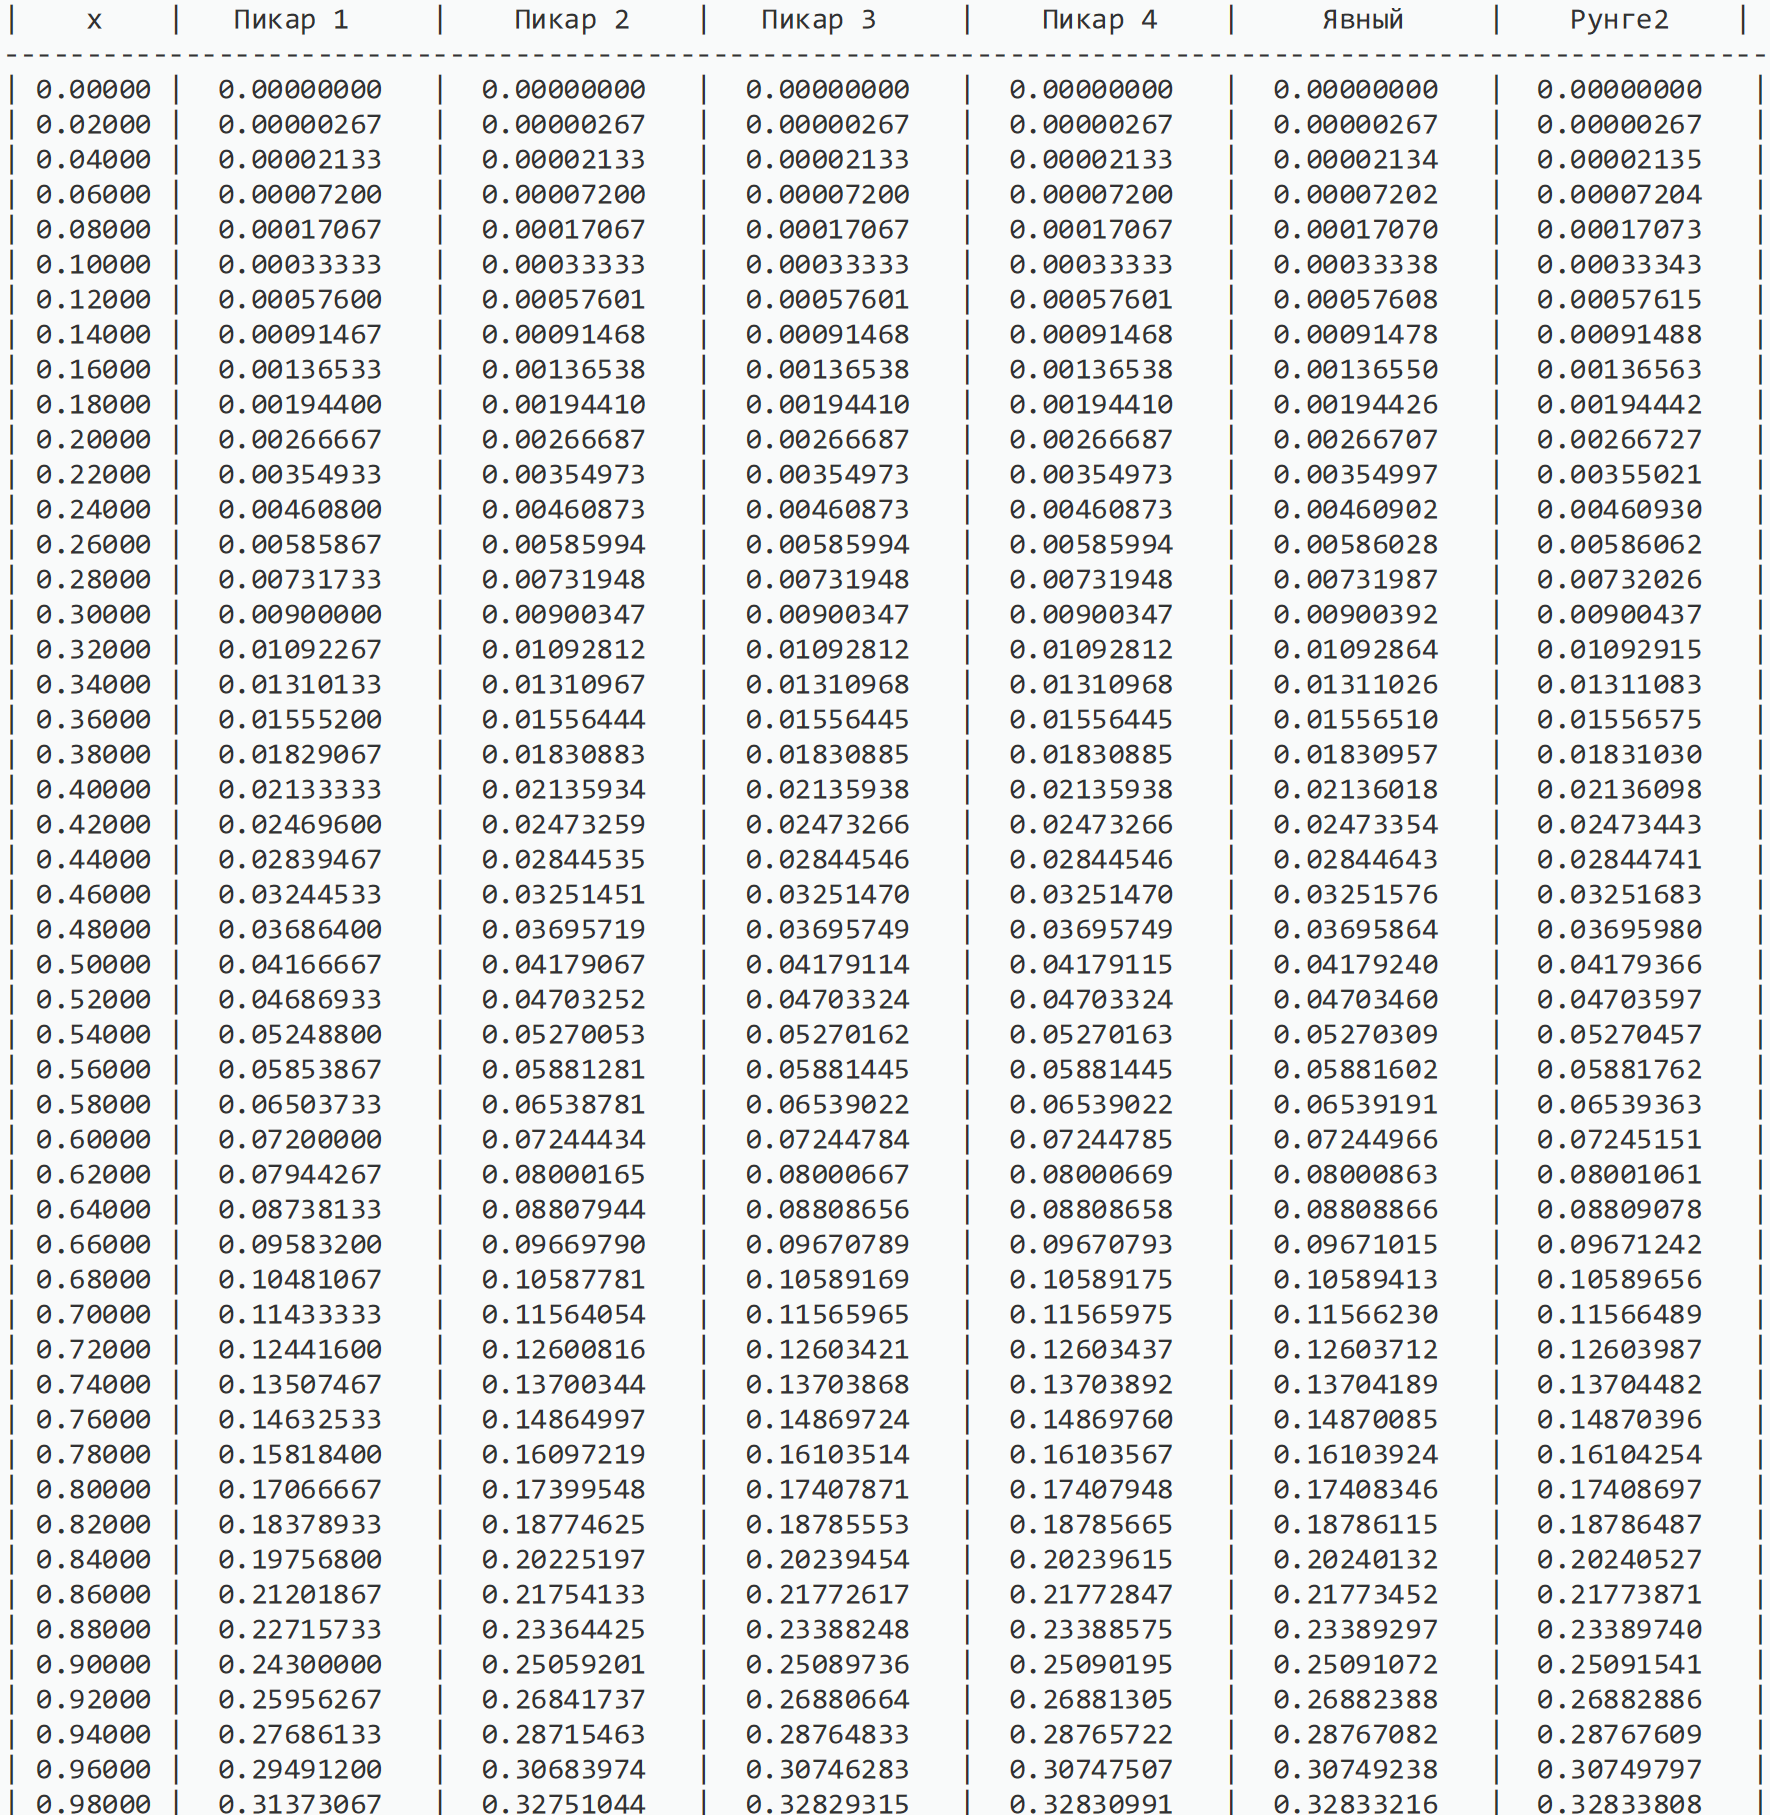
\includegraphics[scale=0.9]{1}
		\centering\caption{пример работы программы}
	\end{figure}
\clearpage
\newpage
	\begin{figure}[h]
		\centering
		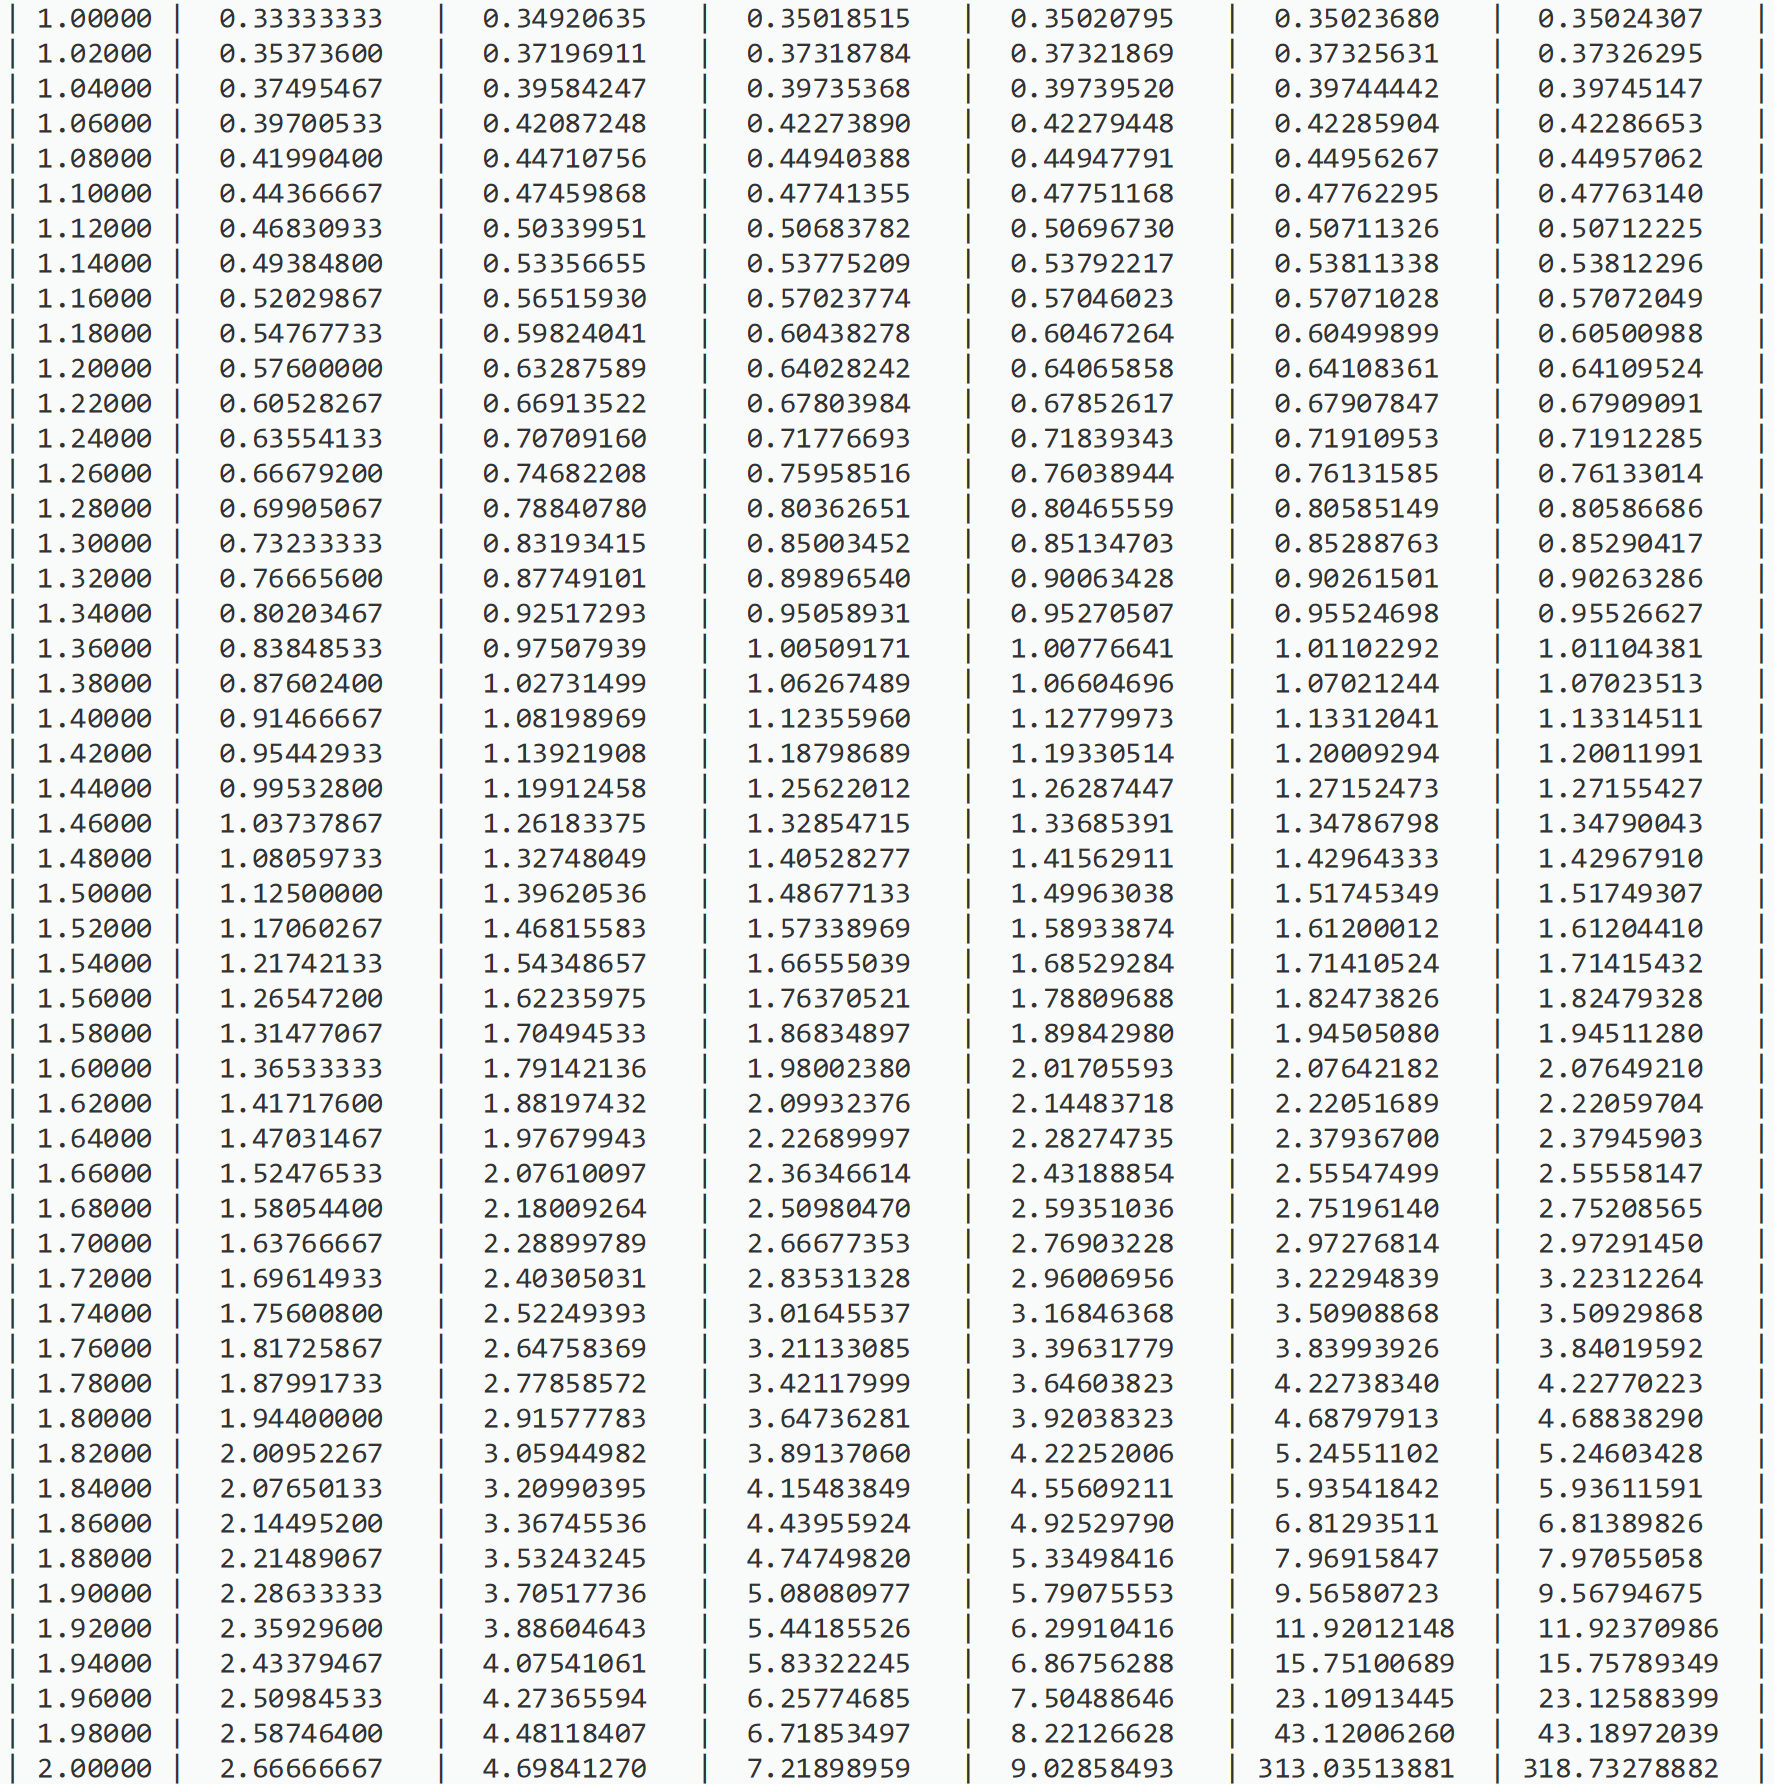
\includegraphics[scale=0.9]{2}
		\centering\caption{пример работы программы}
	\end{figure}

\section{Ответы на вопросы}
\textbf{1) Каково значение функции при x = 2, т.е. привести значение $u$(2)?}
\\Около 313.03.
\\ \textbf{2) Пояснить,  каким  образом  можно  доказать  правильность полученного  результата  при фиксированном значении аргумента в численных методах?}
\\ Сравним результаты в численных методах при значении аргумента равном 2. Чтобы узнать правильность полученного результата, необходимо сравнить результаты численных методов при разном шаге. В нашем случае сравним результаты при шагах: $10^{-3}, 10^{-4}, 10^{-5}, 10^{-6}$. В таблице представлены полученные результаты:

\vspace*{10mm}\hspace*{40mm}\begin{tabular}{ | l | l | l | }
	\hline
	\textbf{Шаг}& \textbf{Эйлер} & \textbf{Рунге-Кутт} \\ \hline
	$10^{-3}$ & 142.62 & 420.28\\ \hline
	$10^{-4}$ & 277.36 & 327.89\\ \hline
	$10^{-5}$ & 313.03 & 318.73\\ \hline
	$10^{-6}$ & 317.24 & 317.82\\ \hline
\end{tabular}
\\ \\ Из этой таблицы можно сделать вывод, что при большом шаге мы получим достаточно грубый и не точный результат в сравнении с результатами при малых шагах. Уже при шагах $10^{-5}, 10^{-6}$, мы получим правльный результат.
\end{document}